%==============================================================================
% Supplementary material for the SIMTiX TVLSI manuscript (simtix_tvlsi.tex).
% Build after the paper (references to it come from simtix_tvlsi.aux via xr):
%   pdflatex simtix_tvlsi && pdflatex simtix_tvlsi_supp && pdflatex simtix_tvlsi_supp
% Parts: supp_figs.tex (ratio figures moved from the paper), supp_lanes.tex (lane
% scaling in full), supp_evalmem.tex (memory-system measurements of the v2 design).
%==============================================================================
\documentclass[journal]{IEEEtran}

\usepackage{cite}
\usepackage{amsmath,amssymb}
\usepackage{graphicx}
\usepackage{booktabs}
\usepackage{xcolor}
\usepackage{xr-hyper}
\usepackage[hidelinks]{hyperref}
\externaldocument[P-]{simtix_tvlsi}

\graphicspath{{../figs/}}
\newcommand{\Fmax}{$F_{\max}$}
\renewcommand{\thesection}{S\arabic{section}}
\renewcommand{\thefigure}{S\arabic{figure}}
\renewcommand{\thetable}{S\Roman{table}}
\usepackage{array}

\begin{document}

\title{Supplementary Material for ``SIMTiX: A Compact RISC-V SIMT Accelerator With
Line-Aggregated Atomic Operations for FPGA Systems-on-Chip''}
\author{Krishna~Gorai and Bikram~Paul}
\markboth{IEEE Transactions on Very Large Scale Integration (VLSI) Systems}%
{Gorai and Paul: SIMTiX, Supplementary Material}
\maketitle

This document holds figures and measurements that support the paper but did not fit
its page budget. Tables, figures and sections without the prefix S are those of the
paper.

\section{Ratios of the Four Machines}\label{sup:ratios}
Figs.~\ref{fig:rodinia} and~\ref{fig:rivec} show, for every Rodinia benchmark and
RiVEC application, the time and the cycles of CVA6, Ara and Vortex, and the time of
the A53, divided by SIMTiX's, from Tables~\ref{P-tab:rodinia} and~\ref{P-tab:rivec}.
Fig.~\ref{P-fig:decomp} of the paper splits these ratios into clock, width and
efficiency.

\begin{figure*}[t]
\centering
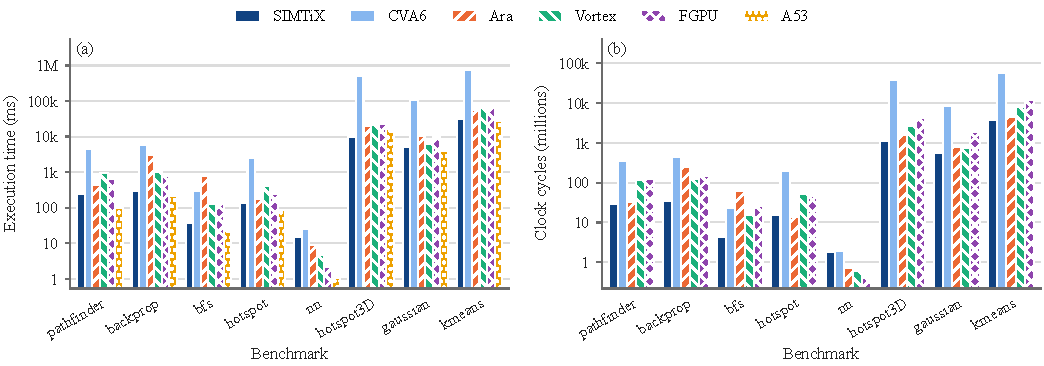
\includegraphics[width=\textwidth]{rodinia_time.pdf}
\caption{Rodinia on the ZCU102. (a) Execution time. (b) Clock cycles.}
\label{fig:rodinia}
\end{figure*}

\begin{figure*}[t]
\centering
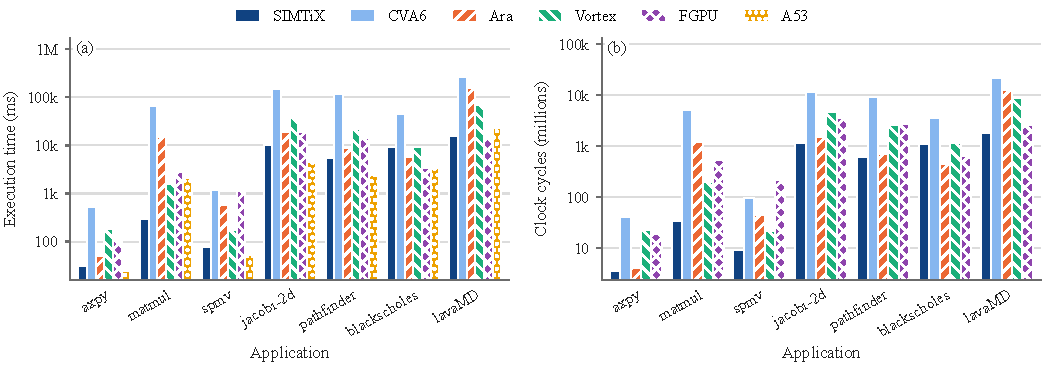
\includegraphics[width=\textwidth]{rivec_time.pdf}
\caption{RiVEC on the ZCU102. (a) Execution time. (b) Clock cycles.}
\label{fig:rivec}
\end{figure*}

\begin{figure*}[t]
\centering
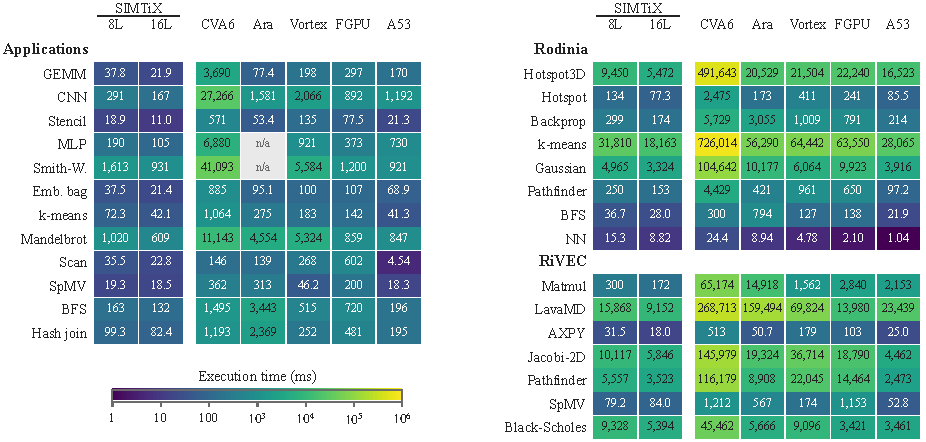
\includegraphics[width=\textwidth]{machines_heatmap_time.pdf}
\caption{Execution time of each machine on the ZCU102.}
\label{fig:mach_time}
\end{figure*}


\section{Out-of-Context Comparison With Vortex}\label{sup:vortex}
Fig.~\ref{fig:vortex} shows, per application, the run time and energy of Vortex at
four, eight and 16 warps relative to SIMTiX, from the out-of-context builds of
Section~\ref{P-sec:evalvortex} and Table~\ref{P-tab:vortex}.

\begin{figure*}[t]
\centering
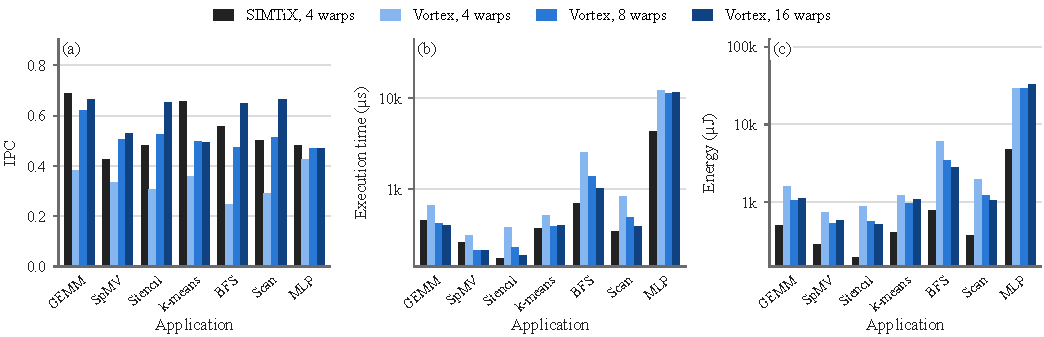
\includegraphics[width=\textwidth]{vortex_metrics.pdf}
\caption{SIMTiX and Vortex out of context. (a) IPC. (b) Execution time. (c) Energy.}
\label{fig:vortex}
\end{figure*}


\section{Scaling With the Lane Count}\label{sup:lanes}
\begin{figure}[t]
\centering
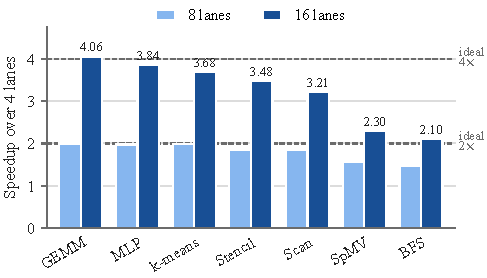
\includegraphics[width=\columnwidth]{lanes_speedup.pdf}
\caption{Speedup of each application at 8 and 16 lanes over a four-lane SIMTiX,
with four warps and a 16~KiB L1 whose line is one word per lane. Dashed lines mark
linear speedup.}
\label{fig:lanes}
\end{figure}

The lane count $L$ is a parameter: it sets the warp width, the line of the memory
engine and the L1 (one word per lane, with the L1 kept at 16~KiB) and the burst
length of the AXI4 master. Fig.~\ref{fig:lanes} shows the speedup over four lanes,
with four warps throughout; all seven applications pass their bit-exact checks at
every lane count. From eight to 16 lanes GEMM gains $2.03\times$, the MLP
$1.95\times$, the stencil $1.88\times$ and k-means $1.86\times$, while scan gains
$1.74\times$, SpMV $1.47\times$ and BFS $1.43\times$. GEMM, the stencil, k-means
and the MLP keep every lane active, and the scan 95\% of them. SpMV and BFS diverge
on their row and neighbor loops, where a warp runs until its longest row or
adjacency list ends, and their lane utilization falls from 66\% and 55\% at four
lanes to 59\% and 43\% at eight and 57\% and 34\% at 16. Their gathers also touch
about one line per lane, and the memory engine sends one request per line: from
eight to 16 lanes the warp instructions of SpMV halve, but its L1 accesses fall
only from 12,100 to 9,625, and its IPC drops from 0.43 to 0.33.

The cost grows faster than the lane count. Four lanes use 43,119 LUTs at
113.5~MHz and eight lanes 84,443 at 101.6~MHz. Placed, the 16-lane design
occupies 190,401 LUTs, 83\% of the XCZU7EV and 2.3 times the eight-lane design,
and 96\% of the device's configurable logic blocks hold some of its logic. Each lane's FPU stays at 4.8k LUTs, but the memory engine,
implemented alone in its board configuration, grows from 4,645 LUTs at four lanes
to 12,576 at eight and 42,474 at 16, by 2.7 and then 3.4 times per doubling; all
three meet 100~MHz. The engine selects the word of every lane from a line that
itself holds one word per lane, places every lane's store data into that line,
and, for the aggregated AMOs, compares the word addresses of every pair of lanes.
These structures grow with the square of the lane count. Wider warps are
therefore limited by the memory engine rather than by the lanes, and beyond eight
lanes more cores, or an engine that serves part of a warp per cycle, are the
better way to add throughput.

The 16-lane run also exposed the stack bound of Section~\ref{P-sec:arch}. Our stack
had eight frames, which by the bound suffices for eight lanes. In SpMV at 16
lanes, a warp whose rows have more than eight different lengths leaves its loop at
more than eight different iterations, pushing a frame each time, and overflowed
the stack. Sizing the stack by the lane count removed the failure; at eight lanes
the design is unchanged.


\section{Sixteen Lanes on the Board, Every Run}\label{sup:lanes16}
Tables~\ref{tab:lanes16_board_all1} and~\ref{tab:lanes16_board_all2} list the 82
board runs of Section~\ref{P-sec:lanes16} of the paper, summarized in
Table~\ref{P-tab:lanes16_board} and Fig.~\ref{P-fig:lanes16_board}: the time of the
Cortex-A53, of the eight-lane design and of the 16-lane design, and the 16-lane design's
speed-up in time and in cycles over the eight-lane design and over the A53. The
eight-lane runs use their own A53 times, measured in the same session.

% generated by sim/compare_board_l16.py from the board logs (2026-11-17)
\begin{table*}[p]
\caption{Sixteen Lanes on the Board: Synchronization Kernels and Applications}
\label{tab:lanes16_board_all1}
\centering\footnotesize
\setlength{\tabcolsep}{4pt}
\begin{tabular}{lrrrrrrrr}
\toprule
Kernel & Input & \multicolumn{3}{c}{Time (ms)} & \multicolumn{2}{c}{16L vs 8L} & \multicolumn{2}{c}{vs A53}\\
\cmidrule(lr){3-5}\cmidrule(lr){6-7}\cmidrule(lr){8-9}
 & & A53 & 8 lanes & 16 lanes & time & cycles & 8L & 16L\\
\midrule
\multicolumn{9}{l}{\textit{Synchronization kernels}}\\
Reduce (shuffle) & 1{,}024 & 0.002 & 0.025 & 0.017 & 1.44 & 1.67 & 0.08 & 0.12\\
Histogram (AMO) & 1{,}024 & 0.008 & 0.025 & 0.019 & 1.28 & 1.51 & 0.33 & 0.43\\
Histogram (shared) & 1{,}024 & 0.008 & 0.039 & 0.028 & 1.38 & 1.61 & 0.21 & 0.29\\
AMO contention & 1{,}024 & 0.021 & 0.148 & 0.125 & 1.18 & 1.37 & 0.15 & 0.17\\
Reduce (shuffle) & 16{,}384 & 0.027 & 0.374 & 0.254 & 1.47 & 1.70 & 0.07 & 0.11\\
Histogram (AMO) & 16{,}384 & 0.125 & 0.352 & 0.273 & 1.29 & 1.49 & 0.36 & 0.46\\
Histogram (shared) & 16{,}384 & 0.125 & 0.638 & 0.427 & 1.50 & 1.73 & 0.20 & 0.29\\
AMO contention & 16{,}384 & 0.352 & 2.32 & 1.98 & 1.17 & 1.35 & 0.15 & 0.18\\
Reduce (shuffle) & 262{,}144 & 0.432 & 5.95 & 4.04 & 1.47 & 1.70 & 0.07 & 0.11\\
Histogram (AMO) & 262{,}144 & 2.00 & 5.65 & 4.34 & 1.30 & 1.51 & 0.35 & 0.46\\
Histogram (shared) & 262{,}144 & 2.00 & 10.26 & 6.78 & 1.51 & 1.74 & 0.19 & 0.29\\
AMO contention & 262{,}144 & 6.18 & 37.20 & 31.70 & 1.17 & 1.35 & 0.17 & 0.20\\
\midrule
\multicolumn{9}{l}{\textit{Applications}}\\
GEMM & 64 & 2.69 & 2.17 & 1.24 & 1.75 & 2.02 & 1.25 & 2.17\\
GEMM & 256 & 170 & 151 & 85.36 & 1.77 & 2.04 & 1.13 & 1.99\\
SpMV & 4{,}096 & 0.479 & 1.14 & 0.935 & 1.22 & 1.40 & 0.42 & 0.51\\
SpMV & 65{,}536 & 18.29 & 20.24 & 18.63 & 1.09 & 1.25 & 0.90 & 0.98\\
Stencil & 128 & 1.34 & 2.73 & 1.59 & 1.72 & 1.99 & 0.48 & 0.85\\
Stencil & 512 & 22.02 & 43.56 & 25.26 & 1.72 & 1.99 & 0.49 & 0.87\\
k-means & 16{,}384 & 2.58 & 7.26 & 4.23 & 1.72 & 1.98 & 0.36 & 0.61\\
k-means & 262{,}144 & 41.32 & 116 & 67.19 & 1.73 & 1.99 & 0.36 & 0.62\\
BFS & 16{,}384 & 4.37 & 9.38 & 7.42 & 1.27 & 1.46 & 0.47 & 0.59\\
BFS & 262{,}144 & 196 & 163 & 132 & 1.23 & 1.42 & 1.20 & 1.48\\
Scan & 65{,}536 & 0.284 & 6.76 & 4.60 & 1.47 & 1.70 & 0.04 & 0.06\\
Scan & 1{,}048{,}576 & 4.54 & 108 & 73.40 & 1.47 & 1.70 & 0.04 & 0.06\\
MLP{,} INT8 & 16 & 46.17 & 11.85 & 6.60 & 1.80 & 2.07 & 3.89 & 7.00\\
MLP{,} INT8 & 256 & 730 & 190 & 105 & 1.80 & 2.08 & 3.85 & 6.94\\
GEMM-RB & 64 & 2.70 & 0.603 & 0.365 & 1.65 & 1.91 & 4.48 & 7.40\\
GEMM-RB & 256 & 170 & 37.73 & 21.91 & 1.72 & 1.99 & 4.50 & 7.74\\
Segmented scan & 65{,}536 & 0.284 & 2.23 & 1.43 & 1.56 & 1.80 & 0.13 & 0.20\\
Segmented scan & 1{,}048{,}576 & 4.54 & 35.48 & 22.84 & 1.55 & 1.79 & 0.13 & 0.20\\
Stencil-RB & 128 & 1.36 & 1.20 & 0.721 & 1.66 & 1.92 & 1.10 & 1.88\\
Stencil-RB & 512 & 22.04 & 18.95 & 10.99 & 1.72 & 1.99 & 1.12 & 2.01\\
k-means-U & 16{,}384 & 2.58 & 4.56 & 2.81 & 1.62 & 1.87 & 0.57 & 0.92\\
k-means-U & 262{,}144 & 41.35 & 72.16 & 42.11 & 1.71 & 1.98 & 0.57 & 0.98\\
SpMV-Z & 4{,}096 & 0.477 & 1.01 & 0.914 & 1.11 & 1.28 & 0.47 & 0.52\\
SpMV-Z & 65{,}536 & 18.25 & 19.34 & 18.50 & 1.05 & 1.21 & 0.94 & 0.99\\
CNN{,} INT8 & 32 & 74.48 & 18.21 & 10.52 & 1.73 & 2.00 & 4.09 & 7.08\\
CNN{,} INT8 & 128 & 1{,}192 & 291 & 167 & 1.74 & 2.01 & 4.10 & 7.13\\
Embedding bag & 256 & 2.05 & 1.28 & 0.732 & 1.74 & 2.01 & 1.61 & 2.80\\
Embedding bag & 4{,}096 & 68.90 & 37.45 & 21.44 & 1.75 & 2.02 & 1.84 & 3.21\\
Hash join & 16 & 1.67 & 1.54 & 1.25 & 1.24 & 1.43 & 1.07 & 1.33\\
Hash join & 22 & 195 & 99.28 & 82.38 & 1.21 & 1.39 & 1.97 & 2.37\\
Mandelbrot & 256 & 53.00 & 68.27 & 42.40 & 1.61 & 1.86 & 0.78 & 1.25\\
Mandelbrot & 1{,}024 & 847 & 1{,}020 & 609 & 1.67 & 1.93 & 0.83 & 1.39\\
Smith-Waterman & 2{,}048 & 129 & 202 & 116 & 1.73 & 2.00 & 0.57 & 1.10\\
Smith-Waterman & 16{,}384 & 1{,}028 & 1{,}613 & 931 & 1.73 & 2.00 & 0.57 & 1.10\\
\bottomrule
\end{tabular}

\end{table*}

\begin{table*}[p]
\caption{Sixteen Lanes on the Board: Suite 2, Rodinia and RiVEC}
\label{tab:lanes16_board_all2}
\centering\footnotesize
\setlength{\tabcolsep}{4pt}
\begin{tabular}{lrrrrrrrr}
\toprule
Kernel & Input & \multicolumn{3}{c}{Time (ms)} & \multicolumn{2}{c}{16L vs 8L} & \multicolumn{2}{c}{vs A53}\\
\cmidrule(lr){3-5}\cmidrule(lr){6-7}\cmidrule(lr){8-9}
 & & A53 & 8 lanes & 16 lanes & time & cycles & 8L & 16L\\
\midrule
\multicolumn{9}{l}{\textit{Suite 2}}\\
Pathfinder & 65{,}536 & 69.76 & 165 & 101 & 1.64 & 1.89 & 0.42 & 0.69\\
Pathfinder & 262{,}144 & 275 & 659 & 402 & 1.64 & 1.89 & 0.42 & 0.68\\
Hotspot & 512 & 37.46 & 55.79 & 32.16 & 1.73 & 2.00 & 0.66 & 1.16\\
Hotspot & 1{,}024 & 152 & 223 & 130 & 1.72 & 1.99 & 0.68 & 1.17\\
Jacobi-2D & 512 & 46.56 & 84.14 & 48.96 & 1.72 & 1.98 & 0.54 & 0.95\\
Jacobi-2D & 2{,}048 & 782 & 1{,}351 & 787 & 1.72 & 1.98 & 0.58 & 0.99\\
ATAX & 1{,}024 & 15.16 & 19.86 & 18.65 & 1.06 & 1.23 & 0.76 & 0.81\\
ATAX & 4{,}096 & 243 & 356 & 401 & \textit{0.89} & 1.03 & 0.68 & 0.61\\
BiCG & 1{,}024 & 15.16 & 19.93 & 17.47 & 1.14 & 1.32 & 0.76 & 0.87\\
BiCG & 4{,}096 & 243 & 357 & 408 & \textit{0.88} & 1.01 & 0.68 & 0.60\\
PageRank & 16{,}384 & 25.07 & 33.35 & 25.83 & 1.29 & 1.49 & 0.75 & 0.97\\
PageRank & 262{,}144 & 909 & 649 & 842 & \textit{0.77} & 0.89 & 1.40 & 1.08\\
Connected comp. & 16{,}384 & 16.82 & 30.94 & 22.31 & 1.39 & 1.60 & 0.62 & 0.75\\
Connected comp. & 262{,}144 & 801 & 623 & 749 & \textit{0.83} & 0.96 & 1.29 & 1.07\\
Backprop & 65{,}536 & 26.80 & 37.42 & 21.71 & 1.72 & 1.99 & 0.71 & 1.23\\
Backprop & 524{,}288 & 215 & 299 & 174 & 1.72 & 1.99 & 0.72 & 1.24\\
Radix sort & 65{,}536 & 16.16 & 65.23 & 100 & \textit{0.65} & 0.75 & 0.25 & 0.16\\
Radix sort & 1{,}048{,}576 & 273 & 1{,}026 & 1{,}584 & \textit{0.65} & 0.75 & 0.27 & 0.17\\
Black-Scholes & 65{,}536 & 27.06 & 112 & 64.60 & 1.73 & 2.00 & 0.24 & 0.42\\
Black-Scholes & 1{,}048{,}576 & 438 & 1{,}790 & 1{,}033 & 1.73 & 2.00 & 0.24 & 0.42\\
\midrule
\multicolumn{9}{l}{\textit{Rodinia}}\\
Pathfinder & 100{,}000 & 97.12 & 250 & 153 & 1.64 & 1.89 & 0.39 & 0.63\\
Backprop & 524{,}288 & 214 & 299 & 174 & 1.72 & 1.99 & 0.72 & 1.23\\
BFS & 65{,}536 & 21.91 & 36.68 & 27.98 & 1.31 & 1.51 & 0.60 & 0.78\\
Hotspot & 512 & 21.00 & 33.55 & 19.34 & 1.74 & 2.00 & 0.63 & 1.09\\
Hotspot & 1{,}024 & 85.47 & 134 & 77.28 & 1.74 & 2.00 & 0.64 & 1.11\\
NN & 42{,}764 & 1.04 & 15.29 & 8.82 & 1.73 & 2.00 & 0.07 & 0.12\\
Hotspot3D & 512 & 16{,}561 & 9{,}450 & 5{,}472 & 1.73 & 1.99 & 1.75 & 3.03\\
Gaussian & 1{,}024 & 3{,}917 & 4{,}965 & 3{,}324 & 1.49 & 1.72 & 0.79 & 1.18\\
k-means & 494{,}020 & 28{,}065 & 31{,}810 & 18{,}163 & 1.75 & 2.02 & 0.88 & 1.55\\
\midrule
\multicolumn{9}{l}{\textit{RiVEC}}\\
AXPY & 2{,}097{,}152 & 25.04 & 31.49 & 18.00 & 1.75 & 2.02 & 0.80 & 1.39\\
Matmul & 512 & 2{,}153 & 300 & 172 & 1.75 & 2.02 & 7.17 & 12.54\\
SpMV & 85{,}623 & 52.75 & 79.22 & 84.02 & \textit{0.94} & 1.09 & 0.67 & 0.63\\
Jacobi-2D & 256 & 4{,}461 & 10{,}117 & 5{,}846 & 1.73 & 2.00 & 0.44 & 0.76\\
Pathfinder & 2{,}048 & 2{,}298 & 5{,}557 & 3{,}523 & 1.58 & 1.86 & 0.45 & 0.65\\
Black-Scholes & 65{,}536 & 3{,}454 & 9{,}328 & 5{,}394 & 1.73 & 2.00 & 0.37 & 0.64\\
LavaMD & 1{,}000 & 23{,}439 & 15{,}868 & 9{,}152 & 1.73 & 2.00 & 1.48 & 2.56\\
\bottomrule
\end{tabular}

\end{table*}



\section{Memory System and Reduction in the v2 Design}\label{sup:evalmem}
We measured the L1 and the memory contexts as they were added, with a set of
synchronization kernels and a memory model of fixed latency. With a 20-cycle
memory, the L1 makes a 16-bin histogram $5.6\times$ faster, its block-shared form
$2.4\times$ and a whole-array sum (a shuffle butterfly and one AMO per warp)
$1.5\times$, while reductions that read each line once change by less than 5\%.
With a 7-cycle memory, four contexts instead of one reduce the cycles of the
whole-array sum by 15\% and of the histogram by 14\%.

In our earlier design without shuffles, a reduction of 1,024 values to one sum
per warp took 6,023 cycles through the scratchpad, 1.38 times the 4,363 cycles of
the same computation on a five-stage RV32I core at the same clock with
single-cycle memory. With a butterfly of three \texttt{shfl.xor} steps, which
leaves the sum in every lane, the reduction takes 2,911 cycles, 1.50 times faster
than that core, and 3,908 cycles behind the L1 and the AXI4 memory model.



\section{Instruction Sets}\label{sup:isa}
Table~\ref{tab:isa} places the SIMTiX instruction set beside the GPU instruction sets
compared in~\cite{vortex}; Section~\ref{P-sec:related} of the paper discusses the
differences.

\begin{table*}[t]
\caption{GPU Instruction Sets and SIMTiX}
\label{tab:isa}
\centering\scriptsize
\setlength{\tabcolsep}{2.2pt}
\renewcommand{\arraystretch}{1.15}
\begin{tabular}{l*{9}{>{\raggedright\arraybackslash}p{0.087\textwidth}}}
\toprule
ISA & Memory model & Threading model & Register file & Thread control &
Synchro\-nization & Flow control & ALU operations & Memory operations & GPU operations\\
\midrule
RDNA & GDS, LDS, constants, global & Workgroup, wavefront, 32/64 threads &
Vector/scalar, 256 VGPRs, 106 SGPRs & End threads, thread mask &
Barrier, wait\_cnt, data dep. & Branch, thread mask & Arithmetic, conditional, bitwise &
Load, store, prefetch & Interpolate, texture sampler\\
GCN & GDS, LDS, constants, global & Compute unit, wavefront, 64 threads &
Vector/scalar, 256 VGPRs, 102 SGPRs & End threads, thread mask &
Barrier, wait\_cnt, data dep. & Branch, thread mask, split/join &
Arithmetic, conditional, bitwise & Load, store, prefetch & Interpolate, texture sampler\\
PTX & Shared, texture, constants, global & Grid/CTA, warp, 32 threads & Scalar &
Predicate & Barrier, membar & Branch, predicate & Arithmetic, conditional, bitwise &
Load, store, prefetch & Texture sampler, load, query\\
GEN & Software managed & Root thread, child thread &
256-bit vector, 128 GRFs, predicate & Send message & Wait, fence &
Branch, SPF registers, split/join & Arithmetic, conditional, bitwise & Load, store &
Interpolate, texture sampler\\
PowerVR & Global, common store, unified store & USC, 32 threads & Vector, 128-bit &
Predicate & Fence & Branch, predicate & Arithmetic, conditional, bitwise & Load, store &
Texture sampler, iteration, alpha/depth\\
Vortex & Shared, global & Compute unit, wavefront & Scalar, 32-bit & Thread mask &
Barrier, flush & Split/join & Arithmetic, conditional, bitwise & Load, store &
Texture sampler\\
\midrule
SIMTiX & Global (L1), block-shared, warp-private & Kernel, block of $2^b$ warps, warp
of 8 threads & Scalar, 32-bit, 32 integer + 32 FP & Hardware spawn, \texttt{ecall},
thread mask & Barrier (\texttt{bar}), RV32A AMOs & Branch, hardware reconvergence
stack & Arithmetic, conditional, bitwise, FP32/FP16, Zba, Zbb min/max, Zicond &
Load, store, line-aggregated AMOs & Shuffle, INT8 dot product (\texttt{pdot8})\\
\bottomrule
\end{tabular}

\end{table*}


\begin{thebibliography}{1}
\bibitem{vortex} B.~Tine, K.~P.~Yalamarthy, F.~Elsabbagh, and H.~Kim,
``Vortex: Extending the RISC-V ISA for GPGPU and 3D-graphics,'' in
\emph{Proc. IEEE/ACM Int. Symp. Microarchitecture (MICRO)}, 2021, pp.~754--766.
\end{thebibliography}

\end{document}
